%KINETIC FRICTION
\newexp \label{exp:kinetic}
  

\section*{Before Lab} In this experiment, we will be investigate the
coefficient of kinetic friction.  In particular, we will measure
the acceleration of a system of masses, and use it to calculate the
coefficient of kinetic friction.

The first step is to derive an expression for $\mu_k$, the
coefficient
of kinetic friction.  You should do this derivation in your lab book
{\em before} you come to lab.  Your TA will check your notebook at
the beginning of the lab.

Here is a sketch of how to go about the derivation.  Consider the block
and pulley system shown in Fig.~\ref{fig:kinetic}.  Draw 
free-body
diagrams (one for each body), identifying all of the forces acting each mass.  Write
Newton's second law for each body.   Assume that the masses are
accelerating.

In class, we have often assumed $\mu_k$ was known and the acceleration
was unknown.
For this experiment, though, you will calculate the
coefficient of kinetic friction using the measured masses and
acceleration.  Consequently, you should solve these equations for the
coefficient of kinetic friction $\mu_k$.  Your
result should be
\setcounter{equation}{0}
\begin{equation}
	\mu_{k} = \frac{mg - (M+m)a}{Mg} \label{eq:kinfric}
\end{equation}
where $M$ and $m$ are the masses as shown in Fig.~\ref{fig:kinetic},
$a$ is the shared acceleration of the bodies, and $g$ is the acceleration
of gravity.

\section*{Introduction and Theory}
In class, we have assumed that the
coefficient of friction is constant---that is, it depends on only on the type of surfaces
in contact, and not on surface area, mass, or other parameters.  In
this lab we will measure the
coefficient of kinetic friction for the same two surfaces, but different
masses, velocities, accelerations, and surface areas, and see whether
or not the coefficient of friction is in fact constant.

Consider Eq.~\ref{eq:kinfric} above.  What does this equation tell us?
We know that the
coefficient of kinetic friction $\mu_{k}$ is assumed to be constant.
If it is, then the left side of Eq.~(\ref{eq:kinfric})
should always have the same value for any condition which results
in motion. 
Hence if we change the masses $M$ or $m$, the acceleration
$a$ should also change, so as to keep $\mu_k$
 the same.
% This makes sense because if a different mass is hung
%on the string it will change the motion of the sliding block.  Keep
%your equations handy in your notebook for later use.

In this experiment, we will use the Pasco computerized data
acquisition system to record the velocity of the falling mass $m$ in
Fig.~\ref{fig:kinetic} as a function of time, and use those data to
find the acceleration of the system.  Given the acceleration and the
masses, we can use Eq.~\ref{eq:kinfric} to find the coefficient of
friction $\mu_k$.

\section*{Apparatus}
Fig.~\ref{fig:kinetic} shows the experimental setup. You should have the following materials
available at your lab station:
\begin{enumerate}
\item Pasco interface box and Smart Pulley (the pulley with wire attached)
\item Table clamp
\item Mass and hanger set
\item Wooden blocks with hooks
\item String
\item Plastic horizontal surface on which the wood block slides
\end {enumerate}
\begin{figure}
\begin{center}
{\resizebox{4.5in}{!}{{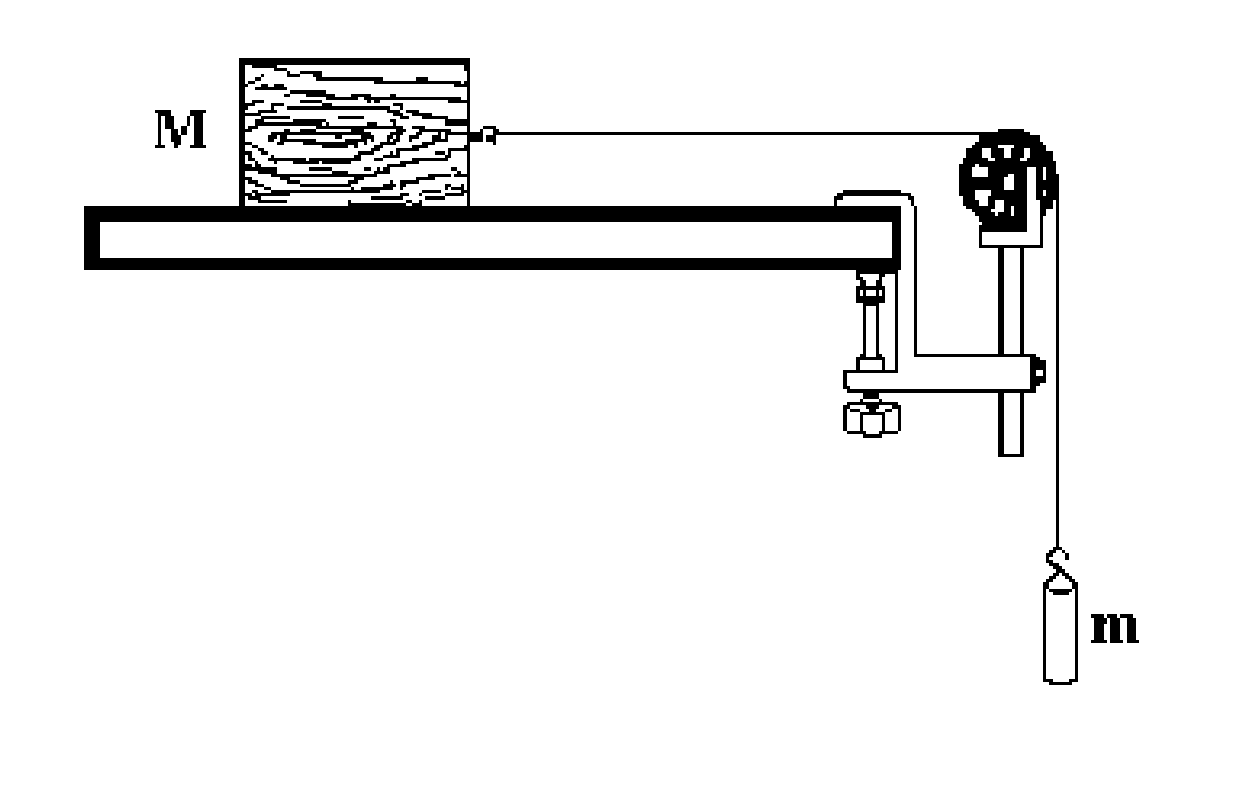
\includegraphics{kineticD.eps}}}}
\end{center}
% \vspace{3.5in}
%   \special{bmp:kinetic.bmp x=4.5in y=3in}
 \caption{Kinetic Friction Apparatus  \label{fig:kinetic}}
\end{figure}
The Smart Pulley should be connected to Digital Channel 1 on the Pasco interface box.
This device reads position by scanning the pulley spokes with a beam
of light.  It thus measures the angular velocity of the pulley.  The
computer uses the radius to convert angular velocity to the linear
velocity of the edge of the pulley---that velocity is of course equal
to the velocity of the descending mass.  All of this is exactly as in
the previous experiment.

\section*{Procedure}
Set up the apparatus as shown in the Figure.  Launch the DataStudio program,
Excel, and a web browser.
%, plug in your Smart
%Pulley, and turn on the computer if it isn't already on.  At this
%point you're ready to run the DataStudio program.  
Your TA
will give you specific instructions on the use of this software.

You will be taking a number of sets of data.  For each set, use the
procedure outlined below:

\begin{enumerate}
%
\item Place enough mass on the hanger so that the block will slide
on the table without needing an initial push (since we are measuring
{\em kinetic} friction).
%
\item Pull the block back until the mass $m$ is raised to the pulley.
Hold the block at rest until the next step.   {\bf Be sure that the string
is level.}
%
\item  When you are ready to take data, click Start in DataStudio and then release the block.
%
\item Now you can view the velocity vs.\ time data on a
DataStudio graph.  Copy and paste the linear portion of these data
to \WAPP and into a spreadsheet (as a backup copy; never print out
this data). Note that data pasted from DataStudio will include
text column labels which need to be deleted from the \WAPP ``Block Copy \& Paste"
web-form. Do a least-squares fit to find
the slope (that is, the acceleration).  You don't need to print the
fit report, but do record the acceleration (and its error) in your spreadsheet and notebook.
Note if the reduced chi-square signals a non-constant acceleration.
(Recall from previous experiment: $\delta v = .003\; {\rm m/s}$ and negligible error in time.)
%
\item For each mass $m$, do \underline{four} separate runs, and find the
acceleration for each.  

Find the average acceleration (spreadsheet function: {\tt average()}) and determine
its error using the standard deviation of the mean (spreadsheet function: {\tt stdev()/sqrt(4)}). Compare the
\WAPP reported errors in $a$ to the error in $a$ determined from
the standard deviation.  Are these error estimates
in the same ballpark (say within a factor of 2)? We will
use these results to find a value for $\mu_k$ (and its error)
for each mass $m$.  
%It may be convenient to save
%your data in a single spreadsheet file, with a separate worksheet page
%for each $m$.
%
\end{enumerate}
Follow the above procedure \underline{three} times
(for a total of 12 runs), each
time for a {\em different} mass $m$, keeping everything else constant.
%For each $m$, take data from four runs.  
Choose your values of $m$ to get
as wide a range of accelerations as possible---that way, we will be
measuring $\mu_k$ under a wide range of experimental conditions.
%

\section*{Data Reduction and Analysis}

For each $m$ calculate a value for $\mu_{k}$ using Eq.~\ref{eq:kinfric} and the average $a$.
Find the error in this $\mu_{k}$ using the ``high-low game" (see page \pageref{par:high.low.game}). 
(Note the maximum value of $\mu_{k}$ is achieved with:
$M^-$, $a^-$, and $m^+$.)
We use this method because a calculation of the uncertainty in
$\mu_{k}$ using the methods of Appendix A is fairly involved.  
This  crude method has
the advantage of simplicity but it
neglects canceling errors.

Make a final results table including $m$, $a$, $\mu_{k}$, and
the uncertainty in $\mu_{k}$.  
Somewhere in the table note the mass of the sliding block ($M$).

You will probably find that the velocity vs.\ time plots are not exactly
linear.  Often there will be a kink where the slope (acceleration)
changes appreciably.  Select such a data set and print out a copy of 
the graph (with fit line).  What do you think caused this behavior?

\subsubsection*{Spreadsheet Calculation}
In this lab you will be repeatedly calculating $\mu_k$ and $\delta \mu_k = (\mu_{k\; \rm high} -\mu_{k\; \rm low})/2$.
You may want to speed these calculations by  entering them as formulas in a spreadsheet.

\begin{center}
\begin{tabular}{|c|c|c|c|c|c|c|c|}
\hline
$M$ & $m$ & $a$              & $\delta a$      & $\mu_{k}$ & $\mu_{k}$ & $\mu_{k}$ & $\delta \mu_{k}$ \\
 (g)& (g) &  ${\rm (m/s^2)}$ & ${\rm (m/s^2)}$ &           & high      &  low      &  \\
\hline
 \phantom{10000}& \phantom{10000}   &  \phantom{10000}& \phantom{10000} & \phantom{10000} &  \phantom{10000}& \phantom{10000} &  \phantom{10000} \\
\hline
  &   &  &  &  &  &  &      \\ \hline
  &   &  &  &  &  &  &      \\ \hline
\end{tabular}
\end{center}

The formulas will depend on which columns contain which values; find below
an example.  (Since your columns may differ from those used in this example,
you need to understand this example, not just copy it!)
\begin{eqnarray}
\mu_k &= & {\tt (B2*9.8-(A2+B2)*C2)/(A2*9.8)}\\
\mu_{k\; \rm high}&=& {\tt ((B2+0.1)*9.8-(A2+B2)*(C2-D2))/((A2-0.1)*9.8)}\\
\mu_{k\; \rm low}&=& {\tt ((B2-0.1)*9.8-(A2+B2)*(C2+D2))/((A2+0.1)*9.8)}
\end{eqnarray}
While entering these formulas may look complex, once completed all further calculations
consist of just entering the data and ``pulling down the cell".

\section*{More experiments}

Do as many of the following additional experiments as time permits.  To save
time do not do the four repetitions to find $\delta a$, instead 
use the \WAPP reported error in $a$ to find $\delta \mu_{k}$.
\begin{enumerate}
\setcounter{enumi}{1}
\item Make another table of $M$, $\mu_{k}$, and $a$ (mass $M$ changing this time).
Do three runs, varying the mass $M$ of
the block each time, but holding the hanging mass $m$ constant.
You can change $M$ by setting masses on the block, but be sure you
start with enough mass $m$ on the hanger that it will always slide.
%In calculating the error in $\mu_{k}$,
%use the \WAPP reported error in $a$ rather than the standard deviation
%of the mean (since you will be doing just one trial for every
%$M$ value).
%
\item  Use masses from your first data set and compare what happens
if you slide the block {\em on its side}.  (Remember to adjust the
pulley height so the string is level!) This experiment will test
whether surface area affects
the kinetic friction coefficient.  Note results in your lab book, comparing the two sets
of data.
%
\item Try to get an estimate of the \underline{static} coefficient of friction
$\mu_{s}$ using the materials provided.
Is it higher or lower than $\mu_{k}$?  Record your results with error.
{\em (Note: you won't need the computer for this part---it's a
simple, but rough, estimate)}
%
%\item Calculate the error in $\mu_{k}$ using the values given by your TA for error in $a$, $m$
%and $M$.  Then compare this to the standard deviation of the mean of your values for $\mu_{k}$
%\item Summarize your results, answer the questions below, and turn in your notebook.
\end{enumerate}

\section*{Conclusions}
Consider your data, including uncertainties, and discuss the
following questions carefully and in detail:

A constant slope for a run implies a constant frictional
force during that run.  Did the frictional force seem to be constant during the runs?

Did the coefficient of friction vary
with acceleration? With surface area? With the mass of the block?

Overall, how good is our assumption that the coefficient of kinetic
friction is constant, within the limits of experimental error?


\section*{Critique of Lab}
     Follow the suggestions given in the Introduction to the
Laboratory Manual.

\section*{Quick Report Card}
Properly report (sigfigs, units, error) your three $\mu_k$ from the first part of the lab.
Record the masses used for the runs in which $\mu_k$ was measured.

%\newpage
%\cleardoublepage
%\begin{center}
% CHECKLIST - Kinetic Friction \\
%\end{center}
%\bigskip
%\begin{center}
%\begin{tabular}{||l|r||}
%ASPECT CONSIDERED & DONE? \\ \hline
%Prelab experiment and proof & \\ \hline
%Table of $m$, $a$, $R$, and $\mu_{k}$ with units and uncertainties & \\ \hline
%Table of $M$, $a$, $R$, and $\mu_{k}$ with units and uncertainties & \\ \hline
%Evaluation of surface area data & \\ \hline
%Summary of results & \\ \hline
%Calculated uncertainties $\delta \mu_{k}$, Compare to $\sigma_{\bar x}$ & \\ %\hline
%Questions answered & \\ \hline
%Cleanup & \\ \hline
%\end{tabular}
%\end{center}
\bigskip
\bigskip
\bigskip

%%COMMENTS:\\
%\newpage
%\newpage
%\bigskip
%\begin{center}
%{\bf Pre-Lab}
%\end{center}
%\centerbmp {4in}{2in}{coin.bmp}
%Perform the following
%mini-experiment: Get a book, a coin, and a ruler.  Place a coin on your closed book.
%Now tilt the book until the coin begins to slide, then lower it until it slides
%down the book at a constant speed. Note this position, then measure
% the angle $\theta$ the book is tilted (by measuring
%two sides of the ``triangle'').  Now calculate the friction coefficient,using
%$\tan \theta = \mu$ and record
% your results.  Question: Is the $\mu$ you just found the Kinetic or Static friction coefficient?  Derive the equation $\tan \theta = \mu$ starting with Newton's Second Law.
%
% {\em Hint: Sum the forces on the coin in the x direction (parallel to the table top), finding the components of N and the frictional
%force.  Then substitute the definition of the frictional force and solve for
%$\mu$.}
%\bigskip
